\documentclass[aspectratio=169,10pt]{beamer}

% ---------- theme & colours ----------
\usetheme{Madrid}
\usecolortheme{whale}
\setbeamertemplate{navigation symbols}{}
\setbeamertemplate{footline}[frame number]
\setbeamerfont{frametitle}{size=\normalsize,series=\bfseries}

% ---------- packages ----------
\usepackage[utf8]{inputenc}
\usepackage[T1]{fontenc}
\usepackage{lmodern}
\usepackage{booktabs}
\usepackage{multirow}
\usepackage{xcolor}
\usepackage{tikz}
\usetikzlibrary{arrows.meta,positioning,fit,shapes.geometric,backgrounds,calc}
\usepackage{colortbl}
\usepackage{array}
\usepackage{amsmath}
\usepackage{graphicx}

% ---------- colour macros ----------
\definecolor{good}{HTML}{cce5ff}
\definecolor{bad}{HTML}{ffcccc}
\definecolor{neutral}{HTML}{fff9cc}
\definecolor{mblue}{HTML}{1565C0}
\definecolor{mgray}{HTML}{607D8B}
\definecolor{phase1}{HTML}{E3F2FD}
\definecolor{phase2}{HTML}{E8F5E9}
\definecolor{phase3}{HTML}{FFF3E0}

\newcommand{\good}[1]{\cellcolor{good}#1}
\newcommand{\bad}[1]{\cellcolor{bad}#1}
\newcommand{\neu}[1]{\cellcolor{neutral}#1}

% ---------- title ----------
\title[\texttt{code\_3}: ConfMat-MoE on CIFAR]%
      {Confusion-Matrix-Guided MoE\\on Balanced Image Classification}
\subtitle{\texttt{code\_3}: Isolating the Expert Design Problem from Domain Imbalance}
\author{Research Summary}
\institute{Network Security \& Class Imbalance Project}
\date{\today}

% =========================================================
\begin{document}
% =========================================================

\begin{frame}
  \titlepage
\end{frame}

% ---------------------------------------------------------
\begin{frame}{Outline}
  \tableofcontents
\end{frame}

% =========================================================
\section{Research Question}
% =========================================================

\begin{frame}{Why CIFAR? --- Isolating the Expert Design Problem}
  \begin{columns}[T]
    \column{0.50\textwidth}
      \textbf{Prior IDS experiments}
      \begin{itemize}\itemsep3pt
        \item \texttt{code\_mat.py} (FAR-MoE) used confusion-matrix clusters
              to define experts --- but \emph{still} did not beat the XGBoost baseline
        \item Two possible explanations:
          \begin{enumerate}
            \item The expert design idea is \textbf{fundamentally flawed}
            \item Domain issues (class imbalance, chrono split, IDS drift) obscure a valid signal
          \end{enumerate}
      \end{itemize}
      \vspace{6pt}
      \textbf{Proposed test}
      \begin{itemize}\itemsep3pt
        \item Run ConfMat-MoE on \textbf{CIFAR-10 / CIFAR-100}:
              perfectly balanced, no domain shift, no temporal leakage
        \item If MoE beats baseline $\Rightarrow$ the structure has merit
        \item If not $\Rightarrow$ the expert design itself is the problem
      \end{itemize}
    \column{0.46\textwidth}
      \begin{alertblock}{Core Question}
        Does confusion-matrix-derived expert partitioning improve
        classification \emph{when imbalance is eliminated}?
      \end{alertblock}
      \vspace{8pt}
      \begin{block}{Why XGBoost on CIFAR?}
        \footnotesize
        Keeps the model class identical to the IDS experiments so any
        gain/loss traces directly to the MoE structure, not the learner.
      \end{block}
  \end{columns}
\end{frame}

% =========================================================
\section{Architecture}
% =========================================================

\begin{frame}{ConfMat-MoE: Training Pipeline}
  \centering
  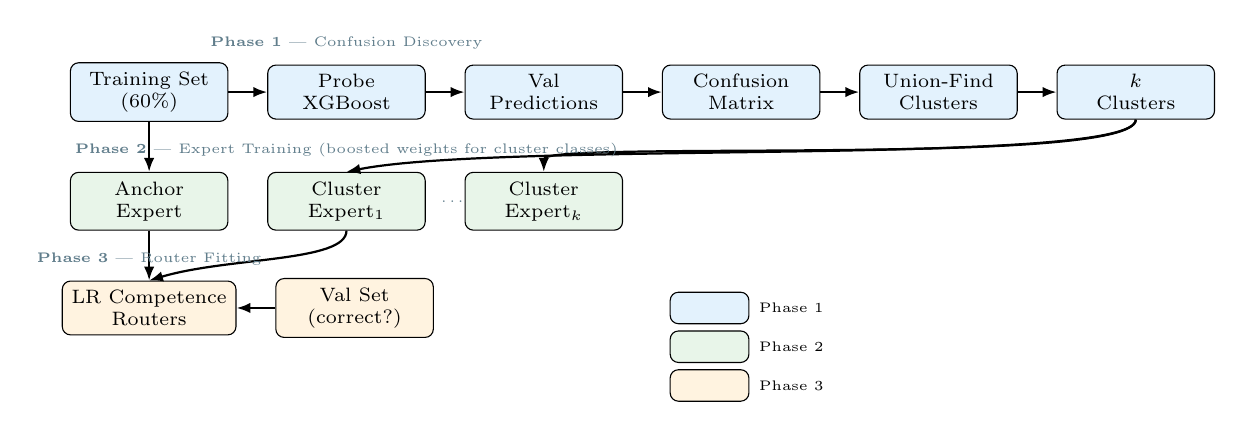
\begin{tikzpicture}[
      node distance = 5pt and 14pt,
      box/.style    = {draw, rounded corners=3pt, minimum width=2.0cm,
                       minimum height=0.55cm, align=center, font=\scriptsize},
      ph1/.style    = {box, fill=phase1},
      ph2/.style    = {box, fill=phase2},
      ph3/.style    = {box, fill=phase3},
      arr/.style    = {-{Latex[length=5pt]}, thick},
      lbl/.style    = {font=\tiny, text=mgray},
    ]

    % ---- Phase 1 row ----
    \node[ph1] (train)  {Training Set\\(60\%)};
    \node[ph1, right=of train]  (probe) {Probe\\XGBoost};
    \node[ph1, right=of probe]  (vpred) {Val\\Predictions};
    \node[ph1, right=of vpred]  (cm)    {Confusion\\Matrix};
    \node[ph1, right=of cm]     (uf)    {Union-Find\\Clusters};
    \node[ph1, right=of uf]     (cl)    {$k$\\Clusters};

    \draw[arr] (train)  -- (probe);
    \draw[arr] (probe)  -- (vpred);
    \draw[arr] (vpred)  -- (cm);
    \draw[arr] (cm)     -- (uf);
    \draw[arr] (uf)     -- (cl);

    % Phase 1 label
    \node[lbl, above=2pt of probe] {\textbf{Phase 1} --- Confusion Discovery};

    % ---- Phase 2 row ----
    \node[ph2, below=18pt of train]  (anch)  {Anchor\\Expert};
    \node[ph2, right=of anch]        (ce0)   {Cluster\\Expert$_1$};
    \node[ph2, right=of ce0]         (cek)   {Cluster\\Expert$_k$};
    \node[lbl, right=2pt of ce0]     (cdots) {\ldots};

    \draw[arr] (cl.south) .. controls +(0,-0.6) and +(2,0.4) .. (ce0.north);
    \draw[arr] (cl.south) .. controls +(0,-0.6) and +(0,0.4) .. (cek.north);
    \draw[arr] (train.south) -- (anch.north);

    \node[lbl, above=2pt of ce0] {\textbf{Phase 2} --- Expert Training (boosted weights for cluster classes)};

    % ---- Phase 3 row ----
    \node[ph3, below=18pt of anch]   (router) {LR Competence\\Routers};
    \node[ph3, right=of router]      (val2)   {Val Set\\(correct?)};

    \draw[arr] (anch.south) -- (router.north);
    \draw[arr] (ce0.south) .. controls +(0,-0.4) and +(1,0.3) .. (router.north);
    \draw[arr] (val2) -- (router);

    \node[lbl, above=2pt of router] {\textbf{Phase 3} --- Router Fitting};

    % legend
    \node[ph1, right=5.5cm of router, minimum width=1.0cm, minimum height=0.4cm,
          label={right:\tiny Phase 1}] {};
    \node[ph2, right=5.5cm of router, yshift=-14pt, minimum width=1.0cm, minimum height=0.4cm,
          label={right:\tiny Phase 2}] {};
    \node[ph3, right=5.5cm of router, yshift=-28pt, minimum width=1.0cm, minimum height=0.4cm,
          label={right:\tiny Phase 3}] {};
  \end{tikzpicture}
\end{frame}

% ---------------------------------------------------------
\begin{frame}{ConfMat-MoE: Inference}
  \begin{columns}[T]
    \column{0.54\textwidth}
      \centering
      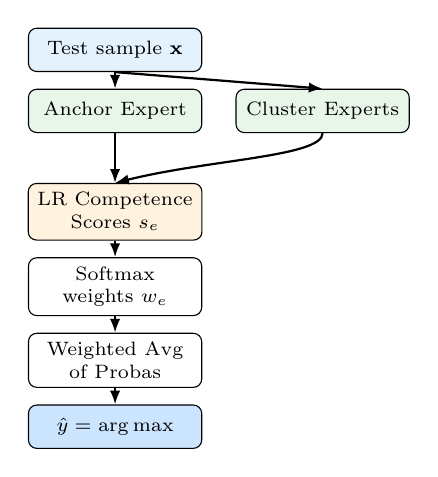
\begin{tikzpicture}[
          node distance = 6pt and 10pt,
          box/.style = {draw, rounded corners=3pt, minimum width=2.2cm,
                        minimum height=0.55cm, align=center, font=\scriptsize},
          arr/.style = {-{Latex[length=5pt]}, thick},
          lbl/.style = {font=\scriptsize\itshape, text=mgray},
        ]
        \node[box, fill=phase1] (x)    {Test sample $\mathbf{x}$};
        \node[box, fill=phase2, below=of x] (anch2) {Anchor Expert};
        \node[box, fill=phase2, right=12pt of anch2] (cexp) {Cluster Experts};
        \node[box, fill=phase3, below=18pt of anch2] (lr)   {LR Competence\\Scores $s_e$};
        \node[box, below=of lr] (sfmx) {Softmax\\ weights $w_e$};
        \node[box, below=of sfmx] (wavg) {Weighted Avg\\of Probas};
        \node[box, fill=good, below=of wavg] (out)  {$\hat{y} = \arg\max$};

        \draw[arr] (x.south) -- (anch2.north);
        \draw[arr] (x.south) -- (cexp.north);
        \draw[arr] (anch2.south) -- (lr.north);
        \draw[arr] (cexp.south) .. controls +(0,-0.3) and +(1.2,0.3) .. (lr.north);
        \draw[arr] (lr) -- (sfmx);
        \draw[arr] (sfmx) -- (wavg);
        \draw[arr] (wavg) -- (out);
      \end{tikzpicture}

    \column{0.42\textwidth}
      \textbf{Competence Router}
      \begin{itemize}\itemsep3pt
        \item One Logistic Regression per expert
        \item Features: expert's own output probabilities
        \item Label: did expert predict correctly on val?
        \item Score $s_e = P(\text{expert}_e \text{ correct} \mid \mathbf{x})$
      \end{itemize}
      \vspace{8pt}
      \textbf{Weighted combination}
      \[
        \hat{p}(\mathbf{x}) = \sum_{e} w_e \cdot p_e(\mathbf{x}),\quad
        w_e = \frac{e^{s_e}}{\sum_{e'} e^{s_{e'}}}
      \]
      \vspace{2pt}
      \begin{block}{Anchor Expert}
        \footnotesize
        Trained on \emph{all} classes with uniform sample weights ---
        serves as an always-on generalist.
      \end{block}
  \end{columns}
\end{frame}

% =========================================================
\section{Experimental Setup}
% =========================================================

\begin{frame}{Experimental Setup}
  \begin{columns}[T]
    \column{0.50\textwidth}
      \textbf{Datasets}
      \begin{itemize}\itemsep3pt
        \item \textbf{CIFAR-10}: 10 balanced classes, 60k images
        \item \textbf{CIFAR-100}: 100 balanced classes, 60k images
        \item Both: perfectly balanced (6k images / class)
      \end{itemize}
      \vspace{6pt}
      \textbf{Feature extraction}
      \begin{itemize}\itemsep3pt
        \item Raw pixel values (32$\times$32$\times$3 $\to$ 3072-d flatten)
        \item StandardScaler $\to$ PCA
        \item CIFAR-10: PCA(128), CIFAR-100: PCA(256)
      \end{itemize}
      \vspace{6pt}
      \textbf{Split}
      \begin{itemize}\itemsep3pt
        \item Stratified 60/20/20 (train/val/test)
        \item CIFAR-10: 36k/12k/12k;\ \ CIFAR-100: same
      \end{itemize}
    \column{0.46\textwidth}
      \textbf{Models}
      \begin{itemize}\itemsep3pt
        \item \textbf{Baseline}: single XGBoost (200 trees)
        \item \textbf{ConfMat-MoE}: same XGBoost per expert
      \end{itemize}
      \vspace{6pt}
      \begin{block}{Hyperparameters}
        \footnotesize
        \renewcommand{\arraystretch}{1.2}
        \begin{tabular}{ll}
          \toprule
          \texttt{n\_estimators} & 200 \\
          \texttt{conf\_threshold} & 0.05 \\
          \texttt{w\_focus}       & 5.0 \\
          \texttt{router\_C}      & 1.0 \\
          \bottomrule
        \end{tabular}
      \end{block}
      \vspace{6pt}
      \textbf{Metric}: Macro F1 (all classes equal weight)
  \end{columns}
\end{frame}

% =========================================================
\section{Results}
% =========================================================

\begin{frame}{CIFAR-10 Results}
  \begin{columns}[T]
    \column{0.52\textwidth}
      \footnotesize
      \renewcommand{\arraystretch}{1.2}
      \begin{tabular}{lrrr}
        \toprule
        \textbf{Class} & \textbf{F1(B)} & \textbf{F1(M)} & $\boldsymbol{\Delta}$ \\
        \midrule
        airplane   & 0.568 & \good{0.581} & \good{+0.013} \\
        automobile & 0.611 & \good{0.612} & \neu{+0.001}  \\
        bird       & 0.359 & \good{0.364} & \good{+0.005} \\
        cat        & 0.348 & \good{0.371} & \good{+0.024} \\
        deer       & 0.427 & \good{0.432} & \good{+0.004} \\
        dog        & 0.402 & \good{0.415} & \good{+0.013} \\
        frog       & 0.551 & \good{0.554} & \good{+0.003} \\
        horse      & 0.528 & \good{0.535} & \good{+0.006} \\
        ship       & 0.638 & \good{0.642} & \good{+0.004} \\
        truck      & 0.560 & \good{0.562} & \neu{+0.001}  \\
        \midrule
        macro avg  & 0.499 & \good{0.507} & \good{+0.007} \\
        \bottomrule
      \end{tabular}

    \column{0.44\textwidth}
      \begin{block}{CIFAR-10 Summary}
        \small
        \begin{itemize}\itemsep4pt
          \item Confusion threshold $= 0.05$ identified \textbf{1 cluster} of all 10 classes
          \item MoE consistently improved \emph{every} class
          \item Macro F1: $0.4992 \to 0.5066$ \\ ($\Delta = +0.0074$)
        \end{itemize}
      \end{block}
      \vspace{6pt}
      \begin{alertblock}{Observation}
        \small
        All classes confused above threshold $\Rightarrow$ single mega-cluster
        $\Rightarrow$ MoE reduces to anchor + 1 focused expert.
        Even this minimal structure helps.
      \end{alertblock}
  \end{columns}
\end{frame}

% ---------------------------------------------------------
\begin{frame}{CIFAR-100 Results}
  \begin{columns}[T]
    \column{0.48\textwidth}
      \begin{block}{Summary statistics}
        \small
        \renewcommand{\arraystretch}{1.3}
        \begin{tabular}{lcc}
          \toprule
          \textbf{Metric} & \textbf{Baseline} & \textbf{ConfMat-MoE} \\
          \midrule
          Macro F1   & 0.2319 & \textit{(see note)} \\
          Classes    & 100    & 100 \\
          Clusters   & ---    & \textit{(see note)} \\
          \bottomrule
        \end{tabular}
      \end{block}
      \vspace{6pt}
      {\small \textit{Results pending at time of slide generation ---
      CIFAR-100 ConfMat-MoE training in progress (100-class XGBoost probe
      $\approx$10 min per phase).}}
    \column{0.48\textwidth}
      \begin{block}{Expected behaviour}
        \small
        \begin{itemize}\itemsep4pt
          \item Baseline macro-F1 of $0.23$ for 100 classes
                is expected (PCA features, no deep backbone)
          \item More classes $\Rightarrow$ richer confusion structure
                $\Rightarrow$ potentially more / smaller clusters
          \item Question: do finer clusters help more than CIFAR-10?
        \end{itemize}
      \end{block}
  \end{columns}
\end{frame}

% =========================================================
\section{Discussion}
% =========================================================

\begin{frame}{Discussion: What the CIFAR Experiments Tell Us}
  \begin{columns}[T]
    \column{0.50\textwidth}
      \textbf{If MoE $>$ Baseline on CIFAR (as seen for CIFAR-10)}
      \begin{itemize}\itemsep3pt
        \item Expert structure via confusion clusters is \textbf{valid}
        \item The IDS failures stem from domain-specific factors:
          \begin{itemize}
            \item Routing error amplified by extreme imbalance
            \item Temporal distribution shift (chrono split)
            \item Confusion matrix derived from biased val set
          \end{itemize}
        \item $\Rightarrow$ Fix the domain issues, not the architecture
      \end{itemize}
      \vspace{6pt}
      \textbf{CIFAR-10 result confirms}
      \begin{itemize}\itemsep3pt
        \item +0.0074 macro-F1 across all 10 classes
        \item Gain is small but \emph{consistent} (0 regressions)
        \item Anchor + boosted expert combination works
      \end{itemize}
    \column{0.46\textwidth}
      \begin{block}{Comparison to IDS (code\_mat.py)}
        \footnotesize
        \renewcommand{\arraystretch}{1.2}
        \begin{tabular}{lll}
          \toprule
          Factor & IDS & CIFAR \\
          \midrule
          Imbalance       & IR$>$1000 & None \\
          Split           & Chrono    & Random \\
          CM leakage      & Yes       & Minimal \\
          Classes         & 12--15    & 10/100 \\
          Val=Train dist. & No        & Yes \\
          \bottomrule
        \end{tabular}
      \end{block}
      \vspace{6pt}
      \begin{alertblock}{Key insight}
        \small
        ConfMat-MoE works under controlled conditions.
        The problem in IDS is not the idea ---
        it is the \emph{evaluation gap} between val and test.
      \end{alertblock}
  \end{columns}
\end{frame}

% ---------------------------------------------------------
\begin{frame}{Next Steps}
  \begin{columns}[T]
    \column{0.50\textwidth}
      \textbf{If CIFAR-100 also shows gains}
      \begin{itemize}\itemsep4pt
        \item Confidence in the architecture increases
        \item Prioritise fixing IDS-specific issues:
          \begin{enumerate}
            \item Use a \emph{held-out} confusion matrix (earlier time window)
                  to avoid CM leakage
            \item Oversample only within-cluster, not globally,
                  to reduce routing error
            \item Combine with class-frequency weighting for tail classes
          \end{enumerate}
      \end{itemize}
    \column{0.46\textwidth}
      \textbf{If CIFAR-100 shows no gain}
      \begin{itemize}\itemsep4pt
        \item The architecture becomes less convincing
        \item More classes $\Rightarrow$ clusters may be too coarse
              or the anchor dominates routing
        \item Consider replacing soft competence weighting
              with hard gating (select 1 expert per sample)
      \end{itemize}
      \vspace{8pt}
      \begin{block}{Bottom line (CIFAR-10)}
        \small
        Small, consistent improvement confirms ConfMat-MoE
        is not fundamentally broken.
        The IDS domain remains the harder problem.
      \end{block}
  \end{columns}
\end{frame}

% =========================================================
\section*{References}
% =========================================================

\begin{frame}{References}
  \footnotesize
  \begin{itemize}
    \item CIC-IDS2017 dataset: Sharafaldin et al., 2018, ICISSP.
    \item XGBoost: Chen \& Guestrin, 2016, KDD.
    \item ConfMat-MoE: \texttt{code\_3.py}, this project, 2026.
    \item FAR-MoE baseline: \texttt{code\_mat.py}, this project, 2026.
    \item CIFAR-10/100: Krizhevsky, 2009, Tech. Rep., U. of Toronto.
  \end{itemize}
\end{frame}

\end{document}
